\documentclass[]{rsos}%%%%where rsos is the template name

%%%% *** Do not adjust lengths that control margins, column widths, etc. ***


%%%%%%%%%%% Defining Enunciations  %%%%%%%%%%%
\newtheorem{theorem}{\bf Theorem}[section]
\newtheorem{condition}{\bf Condition}[section]
\newtheorem{corollary}{\bf Corollary}[section]
%%%%%%%%%%%%%%%%%%%%%%%%%%%%%%%%%%%%%%%%%%%%%%%



\begin{document}

%%%% Article title to be placed here
%\title{Zebrafish survival depends on escaping predators from a distance}
%\title{Enhanced performance in sensing, and not locomotion, improves survival in zebrafish prey}
%\title{Enhanced locomotor performance does not improve survival in zebrafish prey}
\title{A faster escape does not enhance survival: experiments and modeling of prey strategy in zebrafish larvae}


\author{%%%% Author details
Arjun Nair, Christy Nguyen, and Matthew J. McHenry}

%%%%%%%%% Insert author address here
\address{Department of Ecology and Evolutionary Biology\\
University of California, Irvine\\
321 Steinhaus Hall\\
Irvine, CA 92697}

%%%% Subject entries to be placed here %%%%
\subject{Animal behavior, biomechanics}

%%%% Keyword entries to be placed here %%%%
\keywords{pursuit-evasion model, locomotion, predation, sensing, strategy}

%%%% Insert corresponding author and its email address}
\corres{Matthew J. McHenry\\
\email{mmchenry@uci.edu}}



%%%%%%%%%%%%%%% End of first page %%%%%%%%%%%%%%%%%%%%%

\maketitle

%%%%%%%%%% Insert the texts which can accomdate on firstpage in the tag "fmtext" %%%%%

%\begin{fmtext}


\linespread{1.6}\selectfont %Doublespacing


\section*{Abstract}
An escape response is a rapid maneuver that an animal executes to evade predators. 
It is commonly argued, but rarely tested, that this behavior may enhance an animal's survival if performed at greater speed or in a more strategically-favorable direction.
We tested the relationship between locomotor performance and survival in zebrafish (\textit{Danio rerio}) larvae during encounters with predators (adults and juveniles) of the same species.
High-speed 3D kinematics were used to track the body position of prey and predator and to determine the probability of behavioral actions by both fish.
These measurements provided the basis for a probabilistic pursuit-evasion model that simulated the trajectories of the animals, which we verified against measurements of the number of strikes survived by prey.
Contrary to expectation, a parameter analysis of this model found that survival was not improved by increasing the speed or altering the direction of the escape.
Rather, the locomotion of zebrafish larvae operates with sufficient performance due to the relatively slow approach and limited range of the suction feeding employed by fish predators.
We did find that prey survive better when responding from a greater distance, which is an ability that depends on the capacity of the visual and lateral line systems to detect a looming threat.
Therefore, performance in sensing, and not locomotion, is decisive for improving the survival of fish prey.
These results may be applicable to the evolution of predator-prey strategy in a broad diversity of animals.


\section{Introduction}
An escape response allows prey to evade predators with fast locomotion \cite{Bullock:1984gd}.
Because of its potential to directly affect survivorship, natural selection may favor animals that can execute an escape response with high locomotor performance.
Indeed, the physiology and mechanics of locomotion features many traits that are likely adaptations for rapid motion.
Escape responses are controlled by large-diameter command neurons (e.g. the giant axon of squid \cite{YOUNG:1938vi}), which often recruit specialized muscles (e.g. the axial musculature of fish \cite{Eaton:1975ux}), which sometimes animate an appendage that functions only during an escape (e.g. the uropods of crayfish \cite{Johnson:1926cl}).
Prey may direct this escape in an optimal direction \cite{Weihs:1984tb}, or may alternatively benefit from heading in an unpredictable \cite{Humphries:1970hy} or variable \cite{Howland:1974ud} direction.
However, it does not necessarily follow that any improvement in speed or variation in heading will have a positive effect on survivorship.
Fish predators commonly approach their prey at a relatively slow speed \cite{Webb:1984jz,Higham:2007go} and this could permit an escape by prey exhibiting speed and directionality that is sufficiently evasive, but well below physiologically-maximal performance. 
The aim of the present study was to test whether improvements in locomotor performance affect prey survival by examining predator-prey interactions in zebrafish.

We addressed this aim with a novel approach that combines experimentation with an application of pursuit-evasion modelling.
Our methodology was developed to meet the challenges to understanding the coupled dynamics of predators and prey.
This coupling emerges because motion by the prey may (or may not) be in response to the predator, which may (or may not) be a response to prior motion by the prey. 
Regression analyses are generally insensitive to such interdependency, yet may succeed in resolving dominant features of successful prey \cite{Walker:2005vn} or predators \cite{Wainwright:2001ufa}.
It is additionally helpful to study behavioral responses to an artificial predator or prey that is experimentally controlled and therefore not coupled \cite{Gabbiani:1999wz,Stewart:2014cma,Heuch:2007kk,Wainwright:2001ufa,Shifferman:2004fs}.
An alternative approach attempts to formulate a behavioral algorithm of one animal by considering their responses to the measured kinematics of the other.
For example, this technique revealed that predatory bats track evasive moths by maintaining their heading, rather than attempting to anticipate the prey's direction \cite{Ghose:2006dk}. 

The present study also included measurements of predator-prey kinematics, but these provided a basis for modeling the behavior of both the predator and prey.
Our model predicted the trajectories of both animals such that the probability of behavioral actions matched our observations when conducted over number simulations.
This served as a probabilistic, agent-based model with the payout being the number of strikes that the prey survived before capture.
The advantage of an experimentally-validated model is that it allows for an predictive consideration of the effects of differences in behavior on prey survival.

We performed our study on zebrafish (\textit{Danio rerio}). 
The larval stage of this species serves as a model for studying the neurophysiological \cite{Bianco:2015gm,Bagnall:2014iu,Huang:2013vj} and biomechanical \cite{Muller:2004hp,Li:2016cy} basis of behavior.
Predator-prey interactions may be experimentally replicated in the lab, where adults and juveniles strike at larvae with suction feeding and the larvae respond with a fast-start escape response \cite{Stewart:2013bha}.
These are the two principle behaviors that characterize a broad diversity of piscivorous interactions \cite{Weihs:1984tb,Walker:2005vn}. 
When approaching an evasive prey, zebrafish predators approach much more slowly than their maximum speed \cite{Stewart:2013bha}, which is common among suction-feeding fishes \cite{Webb:1984jz,Higham:2007go}.
A slow approach presumably allows greater control over the direction and timing of the suction feeding, which is limited to a brief duration over a small region in front of the mouth \cite{Holzman:2008jc,Holzman:2009uu}. 
The prey, by contrast, respond with an explosive escape response with speed that exceeds that of the predator. 
As suggested by prior experiments \cite{Fuiman:1994td} and pursuit-evasion models \cite{Weihs:1984tb}, the relative speed of predator and prey greatly determines strategy.
We, therefore, performed experiments with juvenile and adult predators with a nearly two-fold difference in body length.


\section{Material and methods}

\subsection{Animal husbandry}
All experiments were conducted on zebrafish (\textit{Danio rerio}, Hamilton 1922) with larvae (5 -- 7 days post fertilization, dpf) that were preyed upon by older fish of the same species. 
To examine how these interactions vary with the size of the predator, we performed one set of experiments using adults ($\geq 9$ months old, Mean $\pm$ 1 SD = $3.4 \pm \SI{0.5}{\cm}$, \textit{N} = 19) and another using juvenile predators ($3-4$ months old, $2.0  \pm  \SI{0.4}{\cm}$, \textit{N} = 19).
All fish were bred from wild-type (AB line) colonies housed in a flow-through tank system (Aquatic Habitats, Apopka, FL, USA) that was maintained at $\SI{28.5}{\celsius}$ on a 14:10 h light:dark cycle. 
To produce larvae, the fertilized eggs from randomized mating were cultured according to standard techniques \cite{Westerfield:UXiBrEuA}.
Predators were motivated to feed by fasting for a period of 7 -- 14 days prior to an experiment.


\subsection{Kinematics}
We arranged the lights and cameras for high-speed recordings of both fish with high-contrast images. 
A hemispherical aquarium ($\oslash = \SI{8.5}{\cm}$) was composed of white acrylic, which served as a translucent diffuser of the IR illumination (940 nm) provided by three lamps (CM-IR200-940, CMVision, Houston, TX, USA), positioned below (Fig. \ref{fig_setup}a). 
These lamps provided high-intensity illumination that was invisible to the fish \cite{Robinson:1993tu}, while visible illumination at low intensity was provided by overhead fluorescent lights.
Each camera (FASTCAM Mini UX50, Precision Photron Inc., San Diego, CA, USA) was fitted with a \SI{55}{\mm} lens (f/2.8 Micro Nikkon AIS, Nikon Inc., Melville, NY, USA) and positioned at a distance that permitted a view of the entire aquarium. 
The cameras were angled above the aquarium to allow both fish to be viewed by at least two cameras when the fish were positioned close together.
The cameras were synchronized to record at a 1,000 fps (at 1024 x 1024 pixels) with a common TTL trigger and controlled with the manufacturer's software (PhotronFASTCAM Viewer).

Predation experiments were performed by recording the swimming of one predator and one prey fish in the aquarium (Fig. 1A). 
This began by placing the fish on opposite sides of a partition.
Following a \SI{15}{\min} acclimation period, we lifted the partition and observed the fish until the predator successfully ingested the prey.
Using a end-trigger to the high-speed cameras, we saved recordings from $\sim \SI{0.5}{\s}$ before the first predatory strike and until $\sim \SI{0.5}{\s}$  after the prey was captured.

Our video recordings were used to perform measurements of 3D kinematics. 
We calibrated the cameras by recording a static body that we constructed with 48 landmarks of known relative position, which was placed in the center of the aquarium.
A direct-linear transform (DLT) was calculated using `Digitizing Tools' software in MATLAB (2015a, MathWorks, Natick, MA, USA) \cite{Hedrick:2008wz} from manually-selected coordinates of these landmarks from the perspective of the three cameras.
Using a custom script in MATLAB, we found the body positions of predator and prey fish by selecting landmarks from two camera views and using the DLT to determine the coordinates in 3D space.
We used the position of the predator's two eyes to calculate a mean position that approximated the buccal cavity (Fig. \ref{fig_setup}a).
The posterior margin of the swim bladder was found on the prey's body, which approximates the center of mass \cite{Stewart:2010ig}.
The initial heading of the prey was approximated by matching an ellipsoid (using the 'regionprops' function in MATLAB) to the body of the prey and measuring the angle of the major axis of the ellipsoid.
All subsequent heading measurements of the prey was defined as the average angular displacement of prey during an escape and was relative to the prior heading of the prey.
We acquired the landmark positions at four key events in each interaction between predator and prey: at (1) the initiation of a predator's approach toward the prey, (2) the middle time point of the duration of suction feeding by the predator and the (3) initiation and (4) completion of the prey's escape response.


\subsection{Descriptive statistics}

Descriptive statistics were used to characterize the probability of actions by the predator and prey during predation experiments.
We recorded the predator-specific parameters of the strike distance ($s$), the distance from the prey at which a strike (i.e. a suction feeding event) was initiated, and the strike duration ($\tau$), which was defined as the period between the opening and closing of the mouth during suction feeding. 
For the prey, we found the reaction distance ($l$), the distance from the predator at which the escape response was initiated.
The prey's kinematics were additionally characterized by the escape angle ($\theta$), the angular change in heading from the resting orientation to the escape path.
The escape duration ($\eta$) included the period for all stages of the C-start and subsequent undulatory swimming, until the larva ceased moving.
The frequency distribution for each of these parameters was found to be well-approximated by the following lognormal probability density function:
%
\begin{equation}%%% Equation lognormal distribution
f(x) = \frac{1}{x\sigma \sqrt{2 \pi}} \text{exp} \left[ -{\frac{(ln(x)-\mu)^2}{2\sigma ^2}} \right],
\label{eqn_lognorm}
\end{equation}
%
where $x$ is a particular behavioral parameter ($s, \tau, l, \theta ,$ or $\eta$), $\mu$ is the log mean, and $\sigma$ is the log standard deviation. 
We determined best-fit values for $\mu$ and $\sigma$ for each behavioral parameter by maximum-likelihood (the `fitdist' function in MATLAB).
Instances where the predator captured the prey, parameters for the prey were not included in the dataset.

The probability that the strike of a zebrafish predator is successful depends critically on the distance between the mouth of the predator and the prey \cite{Stewart:2013bha}.
Strikes were therefore measured as a function of distance.
We binned our distance data using an fixed number of bins and calculated the ratio of number of observations in the bin over the total sample size (Fig. \ref{fig_PDF}\textit{f}).
These binned measurements revealed that the probability of a successful capture $(C)$ was well-characterized by the following sigmoidal function:
%
\begin{equation}%%%Equation for sigmoid function
C(d) = \left[ 1+e^{-r(d-d_0)} \right]^{-1},
\label{eqn_sig} 
\end{equation}
%
where $d$ is the distance between predator and prey, $d_0$ is the decay distance, and $r$ is the decay rate. 
The best-fit values for $d_0$ and $r$ were determined by least-squares (using the `sqcurvefit' function in MATLAB).

All parameters for the prey and predators were compared between experiments with adult predators and juvenile predators.
Because these measurements failed to conform to normal distributions, we performed statistical comparisons using non-parametric statistics.
In particular, we used the two-sample Kolmogorov-Smirnov test (i.e. KS-test) \cite{MasseyJr:1951jo}, which does not assume any particular distribution for the data. 


\subsection{Probabilistic, agent-based model}
A probabilistic, agent-based model was developed to simulate the conditions of our experiments. 
This model predicted the 2D motion of a predator and prey \cite{Isaacs:1965uz} according to algorithms that were specific to the behavioral state of each of these agents (Fig. \ref{fig_setup}b). 
The predator's states were Tracking and Striking and the prey's were Resting and Escaping. 
The duration of states, probability of transitioning between states, and probability of prey capture were determined by random-number generation that conformed to the probability distributions and range of values that we measured.
Therefore, the model treated the predator and prey's actions as probabilistic, but each outcome of an interaction also depended on the determinism of the kinematics of the two agents.
Simulations were scripted in MATLAB to calculate the motion of both agents and their behavioral states, which consequently determined the number of unsuccessful strikes before prey capture.

Each simulation began with the predator in the Tracking state, where it moved at an approach speed with a direction that was always headed toward the prey, with perfect information about the prey's position (Fig. \ref{fig_setup}b). 
If the prey was motionless, then the solver would advance in time to the strike or escape initiation, whichever was found to occur first.
Otherwise, the solver would resolve both predator and prey motion with a fixed time step of \SI{5}{\ms}. 
In this regime, the predator adjusted its heading to track the prey with a temporal time delay, $\lambda$.  
The predator's transition into the Striking state occurred when the prey was within a particular value for the strike distance. 
This value was determined \textit{a-priori} by the generation of a random value (using the `random' function in MATLAB) according to the lognormal probability density function (Eqn. \ref{eqn_lognorm}) for measured values of strike distance.
The capture probability, $C$, for a particular strike depended on the distance between the agents in the middle of a strike, according to our measured parameter values for this relationship (Eqn. \ref{eqn_sig}).
The simulation was terminated if a strike was successful, otherwise the predator reverted to the Tracking state after completion of the strike duration (Fig. \ref{fig_setup}b).
The value of strike duration was determined by the generation of a random value from the lognormal probability density function from measured values.
Single values for the predator speed and delay were used for all simulations (Table \ref{table}) and were determined by trial-and-error to replicate the distribution of the measured number of unsuccessful strikes before prey capture. 
These values were found to approximate measurements reported in prior studies \cite{McHenry:2005tc, Stewart:2013bha}. 

The model simultaneously determined the actions of prey (Fig. \ref{fig_setup}b).
Prey behavior was modeled with Resting and Escaping states because larval zebrafish generally remain still between periods of rapid swimming initiated by an escape response \cite{Stewart:2013bha, Stewart:2014cma}. 
The prey began each simulation in the Resting state, where it was motionless and positioned at a random distance from the predator that was within the aquarium diameter ($\oslash = \SI{8.5}{\cm}$).
The prey transitioned into the Escaping state when the predator moved within the reaction distance, after a latency \cite{Nair:2015gk}.
During an escape, the speed of prey varied as a single saw-toothed pulse, with the maximum value (the peak of the sawtooth) attained at 0.2$\eta$, where $\eta$ is the escape duration. 
We found that this function well-characterized prey speed using a frame-by-frame kinematic analysis of escape swimming for 12 larvae. 
The amplitude of the of the saw-toothed pulse represented the maximum escape speed, $u$, observed in our 12 recordings.
During the escape, the prey was assumed to follow a straight path in a direction determined by the escape angle and escape direction.
The reaction distance, escape angle, and escape duration were determined by random numbers with probability density functions matching experimental measurements.
The escape angle was defined with respect to the prey's frame of reference, with $\theta =  \SI{0}{\degree}$ corresponding to and axis defined by forward motion.
This angle was directed with respect to the right or left side of the body by the escape direction.
The escape direction was defined as the probability that the escape angle was directed toward the side of the body facing away from the predator, with a value (Table \ref{table}) that was previously measured \cite{Stewart:2014cma}.

This model simplified many aspects of the complexity of predator-prey interactions.
It assumed that the kinematics of the two fish may be approximated with two-dimensional motion that is not bounded by an aquarium. 
Simulations were halted if prey successfully escaped on 20 occasions, which reflected the observed maximum and guarded against an errant simulation of infinite duration.
The model's use of random number generation considered the probabilistic effects of biomechanics and neurophysiology without explicitly articulating those elements.
For example, capture success was treated as a distance-specific probability (Eqn. \ref{eqn_sig}) that modeled neither the effects of a predator's suction-feeding hydrodynamics, nor the propulsive forces generated by an escaping prey.
The number of successful escapes before capture for all experiments were compared to the same metric for 1,000 simulations.  
This comparison was executed by a two-sample Kolmogorov-Smirnov test, which was chosen over a Kruskal-Wallis test because of its emphasis on the shape of the distribution.  

We designed a parameter analysis to evaluate the parameters that had the greatest effect on prey survival. 
This was achieved by running monte carlo simulations of the model for a 1,000 simulations where one parameter was varied between -90\% and 100\% of their original mean values at increments of 10\%.
For parameters described by a probability distribution, the log-mean parameter, $\mu$, was adjusted to create the desired percent-change in the mean of the distribution, while $\sigma$ was held constant.
The range of possible random values for each distribution was also adjusted to retain the the same cumulative probability range in the probability distribution.
Each parameter variation yielded 1000 trials, each where the prey has escaped a varying amount of times.
The effect of these manipulations were assessed by comparing the measured number of escapes the prey made against the model's prediction without any parameter variation (\% change = 0) using a Kruskal-Wallis test. 
The results for these comparisons are displayed as escape probabilities in the main text, though the number of escapes plots can be viewed in the supplements (Fig. S2).


\section{Results} %==================================================================

\subsection{Kinematics} %==========
The behavior of both predator and prey were similar whether the predators were juvenile or adult zebrafish.
Prey responded similarly, having indistinguishable differences in escape angle (KS-test: $P = 0.86, N = 164$) and with modest, though significant, differences in reaction distance (KS-test: $P < 0.001, N = 164$) and escape duration (KS-test: $P = 0.04, N = 153$) (Fig. \ref{fig_PDF}\textit{b--c}). 
For example, prey reacted at a mean distance to juvenile predators ($\overline{l} = \SI{0.84}{\cm}, N = 91$), that was about two-thirds the reaction distance to adults ($\overline{l} = \SI{1.26}{\cm}, N = 73$).
Escape swimming lasted for about one-third of a second, with the response to juveniles ($\overline{\eta} = \SI{0.35}{\s}$, $N$ = 91) being only  $\SI{50}{\ms}$ longer than to adults ($\overline{\eta} = \SI{0.30}{\s}$, $N$ = 62).
Prey escaped earlier to adult predators (KS-test: $P = 0.02, N = 89$) by $\SI{41}{\ms}$, on average, relative to the mid-duration of suction feeding.
Juvenile and adult predators were not significantly different in either their strike distance (KS-test: $P = 0.08, \overline{s} = \SI{7.6}{\mm}, N = 154$), or strike duration (KS-test: $P = 0.87, \overline{\tau} = \SI{44}{\ms}, N = 107$) (Fig. \ref{fig_PDF}\textit{d--e}).
Therefore, much of the behavior of predator and prey were similar, despite the fact that the adults were nearly twice the body length of the juveniles.

Despite having similar behavior, adult and juvenile predators differed in capture performance.
Juveniles did not succeed in capturing prey beyond a distance of $\SI{3.2}{\mm}$ ($N = 91$), whereas adults captured prey at a maximum distance that was about 3-times greater ($\SI{10.4}{\mm}, N = 77$).
In the relationship between capture probability and distance (Eqn. \ref{eqn_sig}), the decay distance was used to indicate the spatial range of high capture probability. 
By this metric, the strike of adult predators also exhibited a range that was slightly greater than 3-times the distance of juveniles (Table \ref{table}, Fig. \ref{fig_PDF}\textit{f}).
We tested whether this result was due to juveniles approaching the prey with inferior accuracy by measuring the bearing angle of predators.
This angle corresponds to the radial position of the prey relative to the predator's heading, such that a predator is perfectly accurate for a prey position of $\SI{0}{\degree}$.
The bearing angle when they prey initiated an escape was not significantly different (KS-test: $P = 0.15$) between juveniles ($N = 91$) or adults ($N = 77$).
However, bearing angles changed such that there was a significant difference (KS-test: $P = 0.008$) between adults and juveniles when measured at the moment of mid-gape.
In particular, adult predators succeeded in achieving a median bearing of $\SI{13.1}{\degree}$ (Mean = \SI{35.3}{\degree}), whereas the same metric was $\SI{30.0}{\degree}$ (Mean = \SI{39.2}{\degree}) in juveniles.
This suggests that adults were more accurate in their strikes and more effectively adjusted their heading in the time between escape and strike.


\subsection{Probabilistic, agent-based model} %==========
The trajectories of predator and prey fish followed paths that were qualitatively similar to that predicted by our pursuit-evasion model.
For most of the duration of our experiments, predators were observed to be swimming toward the prey (Fig. \ref{fig_traj}a). 
In contrast, the prey were generally motionless, except  when executing escape swimming.
The predators and prey followed a more circuitous path in the predation experiments than the motion prescribed by our model (Fig. \ref{fig_traj}b).
Nevertheless, the temporal sequence of events in the model offered a reasonable approximation of the kinematics of live predator-prey interactions.

The model accurately predicted the broad quantitative patterns of our experimental results.
This was assessed by the probability of the prey surviving over a particular number of strikes. 
In our experiments, prey exhibited the greatest probability of being captured on the first strike with monotonically decreasing probabilities over subsequent strikes (Fig. \ref{fig_traj}c).
Adults were more successful on the first, second and third strikes than juveniles, which consequently exhibited a more even probability distribution.
The model was successful in replicating these trends, which were found to be statistically indistinguishable for both adult (KS-test: $P = 0.93, N = 73$) and juvenile (KS-test: $P = 0.86, N = 91$) predators. 
Furthermore, all trends from the parameter analyses of the pursuit-evasion model were similar between the adult (Fig. \ref{fig_sense}) and juvenile (Fig. S1) predators. 

A parameter analysis of prey parameters revealed that escape speed and reaction distance were the only parameters with a substantial effect on prey survival. 
This result was determined by adjusting the probability distribution of each parameter to generate a percent change in the mean value of that parameter among 1,000 simulations.
Generating these changes in escape duration, escape direction, and escape angle led to statistically insignificant or small changes in escape probability (Fig. \ref{fig_sense}a). 
An increase in escape speed similarly had a negligible effect on survival, but survival probability did decline when speed was reduced by 50\% or more.
However, survival was most sensitive to reaction distance.
Increases to the mean reaction distance caused escape probability to increase up to 16\% and decreases in the mean reaction distance by 30\% or more had a dramatic adverse effect on survival (Fig. \ref{fig_sense}a). 

We examined how the effect of reaction distance varies with escape speed by conducting a two-dimensional parameter analysis (Fig. \ref{fig_sense}\textit{b}).
It was not until speed was reduced by more than 50\% that the relationship between response distance and survivor was altered.
For example, reducing speed by 70\% yielded a distinct curve, the shape of which was similar to the sigmoid generated at higher speeds (Fig. \ref{fig_sense}\textit{c}). 
Alterations in response distance did affect the relationship between escape speed and survival, though the shape of this curve was largely unaltered (Fig. \ref{fig_sense}\textit{d}).
This suggests little evidence for an interactive effect on survival between escape speed and response distance.

\pagebreak

\section{Discussion}%================================

We found that the survival of larval fish does not increase by escaping at a faster speed or by varying direction, but only by responding from a greater distance.
These results were attained through a parameter analysis of a model (Fig. \ref{fig_setup}\textit{b}) that calculated the trajectories of predator and prey and the outcome of predatory strikes (Fig. \ref{fig_traj}\textit{a,b}). 
This probabilistic, agent-based model successfully replicated the broad patterns of survival (Fig. \ref{fig_traj}\textit{c}) by simulating behavioral actions that matched our measurements (Fig. \ref{fig_PDF}).
Our analysis of its predictions suggests that prey survival in fishes may be enhanced by increasing the performance of sensing and not locomotion.

\subsection{Locomotor performance and prey survival} 

The survival of prey depends largely on the actions of the predator.
In contrast to the explosive speed of an escape response \cite{Muller:2004hp}, zebrafish predators tend to approach their prey substantially slower than their capacity, often by braking \cite{McHenry:2005tc}.
The approach speed amounted to less than one-third the maximum speed of escaping larvae (Table \ref{table}), which is consistent with previous measurements \cite{Stewart:2013bha}.
The approach speed relates strategically to the mechanics of feeding.
The suction feeding of fishes succeeds in capturing prey in only a small region around the mouth over a duration of merely tens of milliseconds \cite{FerryGraham:2003bz,Higham:2005kg,Holzman:2007p15907}.
A slow approach is common among suction-feeding fishes and is likely a means of enhancing strike accuracy \cite{Webb:1984jz,Higham:2007go}.
This style of predation is seen over many spcecies of fish \cite{Higham:2007hy}.
Furthermore, our data suggest that zebrafish predators are more likely to capture predator when approaching larval zebrafish with slower approach speeds (Fig. S3).
Therefore, the limited range of suction feeding may constrain some predators to a slow approach while offering prey an opportunity to escape \cite{Holzman:2009uu}.
Despite this strategic advantage for prey, adult zebrafish captured prey on the first strike more than one-quarter of the time and rarely needed more than three strikes to be successful (Fig. \ref{fig_traj}\textit{c}).

The effectiveness of an escape has previously been considered by classic pursuit-evasion models of fish predation.
Classic models resolve how the direction of an escape affects the distance between predator and prey with analytical mathematics \cite{Isaacs:1965uz,Weihs:1984tb}. 
They generally model a single encounter and assume that both animals move with a fixed heading and speed over time. 
A recently-developed version predicted that animals like zebrafish operate in a `slow-predator' domain, where the predator moves more slowly than the prey \cite{Soto:2015cj}.
In this domain, no optimal escape angle exists and prey may rather evade predators with a broad range of escape directions and this range is only modestly expanded by a faster escape. 
In contrast, the predator gains a strategic advantage when the approach at a faster speed than the prey's escape\cite{Weihs:1984tb}. 
Consistent with these ideas, we found a monotonic decrease in survival as we reduced escape speed below half of the observed value (Fig. \ref{fig_sense}\textit{a}) in our simulations. 
In addition, we found only modest differences in survival between experiments using adult and juvenile predators (Figs. \ref{fig_PDF},\ref{fig_traj}\textit{c}), despite a nearly two-fold difference in body size.
This would also be expected by classic theory because the interactions operate in the slow-predator domain in both cases.
It follows from this theory that prey strategy benefits greatly by escaping faster than the predator, but further increases in speed offer diminishing returns.

Granted, in the 'fast-predator' domain, it could be postulated that there could be profound differences in the results from our model.
Studies have shown that the kinematics of an escape response matter greatly when escaping predators \cite{Howland:1974ud, Domenici:2001gj}.
For example, in classical pursuit-evasion models, the escape angle is a critical parameter for survival \cite{Weihs:1984tb}.
Furthermore in situations when the predator is faster than the prey, prey adapt other behaviors, such as shoaling, as a predator defense \cite{pitcher:1986}.
However, these studies do no consider the effect of sensation can have on prey survival.
Currently, our model cannot address this domain of predator-prey interactions.
However, future studies with the presented model could examine how  important the kinematics of escape are relative to sensation.

The strategic conditions exemplified by zebrafish have the potential to be applicable to a diversity of fish species, but represent a special case among predator-prey interactions.
Suction feeding is ubiquitous among fishes and a slow approach is common \cite{Webb:1984jz,Higham:2007go}.
However, not all fish predators are slower than the prey.
Ram-feeding fishes strike at prey while swimming at a relatively high speed and may thereby place prey at a strategic disadvantage.
Success in ram feeding may, in-turn, require superior coordination in directing and timing a strike \cite{Wainwright:2001ufa}.
Ram feeding therefore shows greater similarly in strategy to flying predators such as birds \cite{Shifferman:2004fs}, bats \cite{Ghose:2006dk}, and insects \cite{Combes:2012et}.
In these systems, the escape direction emerges as an important factor in prey strategy \cite{Domenici:2011tv,Domenici:2011vl}.
This direction may conform to an optimal value \cite{Weihs:1984tb}, or may benefit prey by being unpredictable \cite{Humphries:1970hy}.
Other factors, such as the turning radius of an escape trajectory \cite{Howland:1974ud}, or the rate of changes in direction \cite{Humphries:1970hy} additionally become important when the predator is faster than the prey. 


\subsection{Prey survival depends on reaction distance} 

The reaction distance has broad strategic significance.
The predictions of pursuit-evasion models support the simple notion that prey are more evasive if they start from further away \cite{Soto:2015cj,Isaacs:1965uz,Weihs:1984tb}.
This principle is consistent with evolutionary models that contrast the fitness benefit of responding from a distance against its potential costs \cite{Cooper:2015vf,Ydenberg:1986tm}.
For example, escape responses that are initiated at high frequency may be energetically expensive, prohibit foraging, or succeed in revealing cryptic prey \cite{Broom:2005gq}.
Responding from a great distance may even be inferior on purely strategic grounds.
A prey that is slower than a predator, but capable of executing a tight turn, may benefit from initiating this maneuver at the final moments of a predatory strike \cite{Howland:1974ud}.
Therefore, a greater response distance offers a clear strategic benefit in zebrafish (Fig. \ref{fig_sense}), but may not be universally advantageous.

The primacy of reaction distance underscores the strategic importance of predator detection. 
Fish sense water flow with the mechanosensory lateral line system and this sensory modality is necessary for zebrafish larvae to survive predation \cite{Stewart:2013bha}.
The bow wave of flow generated ahead of a gliding predator succeeds in triggering a fast start in zebrafish larvae within a distance of \SI{1.3}{\cm} \cite{Stewart:2014cma}, which is a range that includes many of the responses that we recorded (Fig. \ref{fig_PDF}\textit{c}).
Although flow-mediated responses permit a close approach by the predator, the response is rapid and may trigger an escape in less than $\SI{10}{\ms}$  \cite{Liu:1999fs}. 
Escape responses may also be elicited by a looming visual stimulus \cite{Bianco:2011ca}, but the demands for visual processing necessitate a latency of at least $\SI{200}{\ms}$ \cite{Burgess:2007vp}. 
Nonetheless, the greatest reaction distances that we observed were likely generated by the visual appearance of the predator.
Therefore, the visual system offers prey fish the means to enhance survival by responding to a predatory threat from a distance (Fig. \ref{fig_sense}).
Vision and flow-sensing may be augmented by olfactory cues \cite{Waldman:1982ic}, though zebrafish do not acquire a sensitivity to the alarm pheromone Schreckstoff until a later stage of growth (>48 dpf) \cite{Waldman:1982ic}.


\subsection*{Summary} 

We found that zebrafish larvae operate in a slow-predator strategic domain when preyed upon by adults and juveniles of the same species.
As a consequence, increasing the speed or varying the direction of an escape response shows a negligible effect on survival (Fig. \ref{fig_sense}.
Survival may instead be enhanced by initiating the escape from greater distance by rapidly identifying the predator as a threatening visual stimulus.  
These findings offer valuable insight into the key strategic factors that govern predator-prey interactions in a diversity of fishes and other animals that operate with a similar strategy. 



%\section*{Data accessibility}


\section*{Authors' contributions}

The study was designed in collaboration between AN and MJM.
AN and CN performed all experiments and kinematic analysis.
The probabilistic, agent-based model was created by AN, with guidance from MJM. 
The manuscript was written collaboratively by AN and MJM.

\section*{Competing interests}

We declare we have no competing interests.

\section*{Funding}

This research was supported by grants to MJM from the National Science Foundation (IOS-1354842) and the Office of Naval Research (N00014-15-1-2249).

%\section*{Acknowledgments}
%Insert the Acknowledgment text here.


%\end{doublespace}

%%%%%%%%%% Insert bibliography here %%%%%%%%%%%%%%
%\section*{References}

\linespread{1}\selectfont %Single spacing

\bibliography{ref}
\bibliographystyle{prsb}   %References the PRSB style file

\pagebreak



\section*{Figures \& Tables}

\linespread{1.3}\selectfont %Single spacing

\begin{table}[!h]
\scriptsize
%\small
%\tiny
%\fontsize{6}{6}
\caption{Behavioral parameters and probability distributions}%%%Table caption goes here
\begin{tabular}{lllll}%%%The number of columns has to be defined here
\hline
Variable &State &Adult predator & Juvenile predator\\
\hline
\textit{Predator}& & & & \\
Approach speed, $U$ ($\SI{}{\m\s} ^{-1}$) &T &$U = 0.13$ & $U = 0.05$ \\
Predator delay, $\lambda$ (ms) &T &$\lambda = 10$ &$\lambda = 10$ \\
Strike distance, $s$ (m) &T $\to$ S &$\mu_d$ = -4.980, $\sigma_d$ = 0.448 (\textit{N} = 51) & $\mu_d$ = -5.100, $\sigma_d$ = 0.648 (\textit{N} = 103)\\
Strike duration, $\tau$ (s) &S &$\mu_{\tau}$ = -3.166, $\sigma_{\tau}$ = 0.331 (\textit{N} = 53) & $\mu_{\tau}$ = -3.208, $\sigma_{\tau}$ = 0.399 (\textit{N} = 54) \\
Capture probability, $C$ &S &\textit{r} = \SI{0.573}, \textit{$d_0$} = \SI{5.20}  (\textit{N} = 77) &\textit{r} = \SI{1.99}, \textit{$d_0$} = \SI{1.60}  (\textit{N} = 91) \\ \\
%%
\textit{Prey}& & & & \\
Reaction distance, $l$ (m) &R $\to$ E &$\mu_l$ = -4.546, $\sigma_l$ = 0.587 (\textit{N} = 73) &$\mu_l$ = -4.941, $\sigma_l$ = 0.582 (\textit{N} = 91) \\
Escape angle, $\theta$ (rad) &E  &$\mu_{\theta}$ = 0.144, $\sigma_{\theta}$ = 0.449 (\textit{N} = 206) &$\mu_{\theta}$ = 0.144, $\sigma_{\theta}$ = 0.449 (\textit{N} = 206) \\
Escape duration, $\eta$ (s) &E &$\mu_{\eta}$ = -1.369, $\sigma_{\eta}$ = 0.552 (\textit{N} = 62) &$\mu_{\eta}$ = -1.167, $\sigma_{\eta}$ = 0.5234 (\textit{N} = 91) \\
Escape direction, $\upsilon$ &E &$\upsilon=0.696$ (\textit{N} = 206) &$\upsilon=0.696$ (\textit{N} = 206) \\
Escape latency, $\chi$ (ms) &E &$\chi = 8$ (\textit{N} = 15) & $\chi = 8$ (\textit{N} = 15)\\
Escape speed, $u$ ($\SI{}{\m\s} ^{-1}$) &E  &$u = 0.4$ (\textit{N} = 12) &$u = 0.4$ (\textit{N} = 12) \\\hline
\label{table}
\end{tabular}

T, Tracking; S, Striking; R, Resting; E, Escaping; $\mu$, log mean; $\sigma$, log standard deviation; $r$, decay rate (\SI{}{\per\mm}); $d_0$, decay distance (\SI{}{\mm}).
\end{table}%%%End of the table

\pagebreak

\linespread{1}\selectfont %Single spacing

%The output for figure is:

\begin{figure}[!h]
\centering
	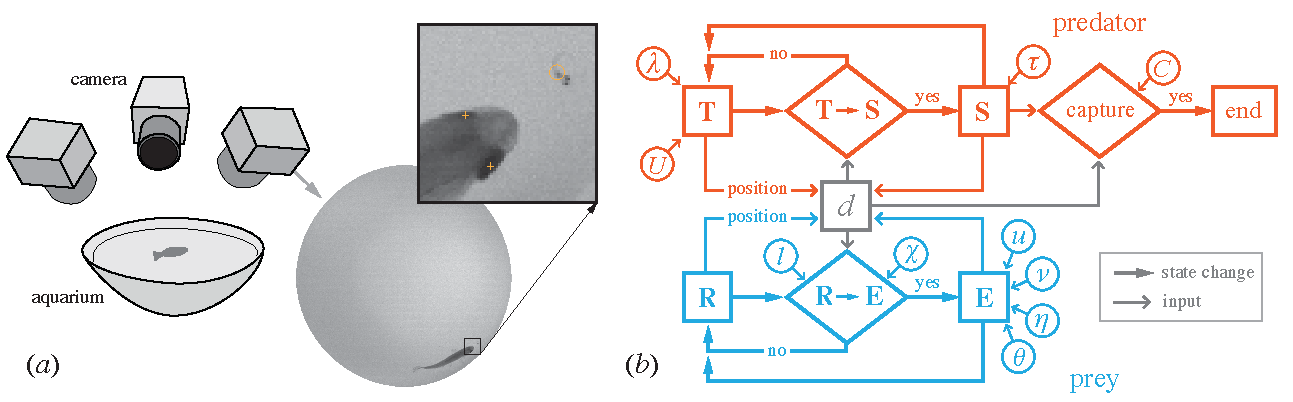
\includegraphics[width=5.5in]{fig_setup}
\caption{
Kinematic measurements and probabilistic, agent-based modeling for studying predator-prey interactions in zebrafish. 
(\textit{a}) Three high-speed video cameras recorded video of one larval prey and one predator fish (adult or juvenile) that were placed in a hemispherical aquarium. 
A representative video frame (cropped to the margin of the aquarium) shows an adult in close proximity to the prey. 
In the inset, orange markers denote the locations of morphological landmarks used to describe the position of the two fish.
This consisted of the position of the two eyes for the predator ("+") and the posterior margin of the swim bladder in the prey (open circle). 
 (\textit{b}) A flow chart illustrates the major components of the model used to simulate the interactions between predators and prey (see Table \ref{table} for symbol definitions and parameter values). 
Each fish behaves according to an algorithm is specific to a particular behavioral state and the probability of transitioning between states is determined by random-number generators with probability distributions matching kinematic measurements (Fig \ref{fig_PDF}).
Predators (in red) operate between Tracking (T) and Striking (S) states and prey are either Resting (R) or Escaping (E).
The outcome of a strike is determined by the capture probability ($C$, Eqn. \ref{eqn_sig}). 
See Materials and methods for details.
 }
\label{fig_setup}
\end{figure}

\pagebreak

\begin{figure}[!h]
\centering
	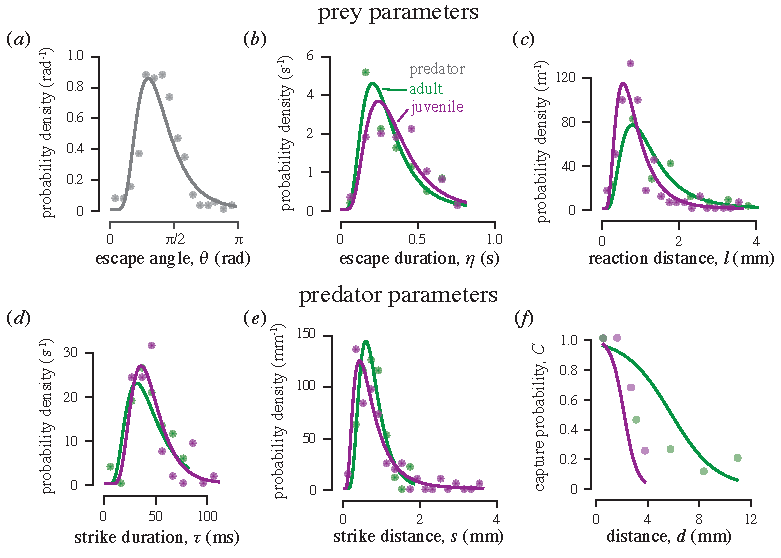
\includegraphics[width=5.5in]{fig_PDFs}
\caption{
Descriptive statistics of swimming kinematics. 
(\textit{a-e}) The probability measurements (circles) and probability density function (Eqn. \ref{eqn_lognorm}) fits for experiments where the predator was a juvenile (purple) or adult (green) predator.
Parameters were measured from the kinematics of prey (\textit{a-c}) and predators (\textit{d-e}) (See table 1 for sample sizes).
Points on graph denotes measured probability density.
Each point represents a bin of the respective data and the size of the bins were determined using the Freedman-Diaconis rule.
The value of each bin is the probability density and is calculated as the ratio of the number of observed samples of data in the bin over the product of the total sample size and the bin width.
The curves represent the continuous, least squares fit to the discrete data.
(\textit{f}) The capture probability was examined as it varies with distance between the predator and prey (Eqn. \ref{eqn_sig}).  
}
\label{fig_PDF}
\end{figure}

\pagebreak

\begin{figure}[!h]
\centering
	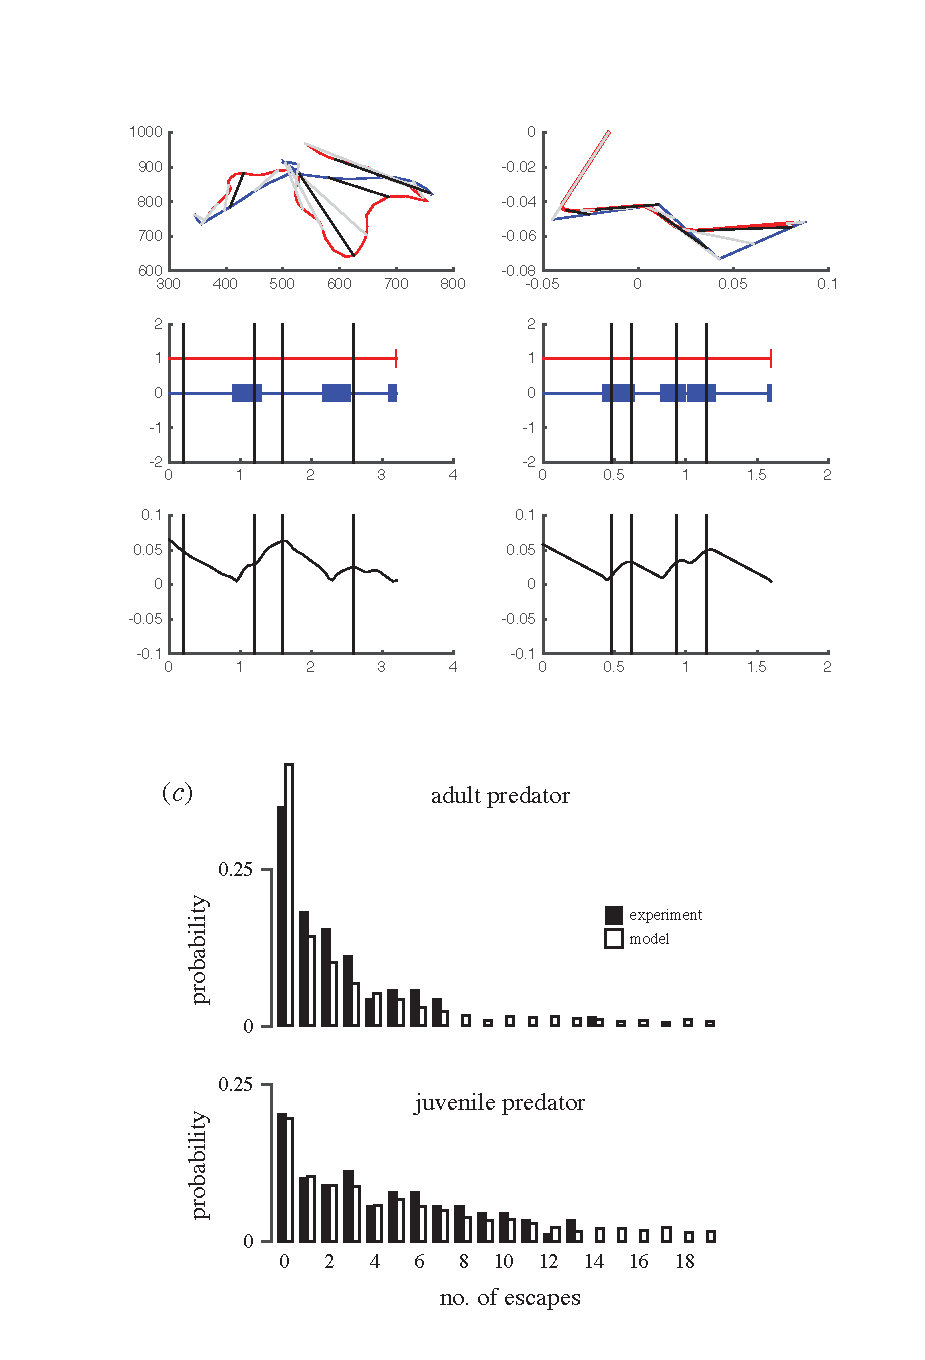
\includegraphics[width=4.5in]{fig_trajectories}
\caption{
Comparison between experimental measurements and modeling. 
(\textit{a}) Trajectories of predator and prey from a representative experiment (left) and simulation (right). 
The position of predator and prey that correspond to particular time points are shown with connecting arrows.
(\textit{b}) Ethograms for these trajectories illustrate the temporal changes in the predator's swimming and strike (left), which are respectively modeled by the Tracking (T) and Striking (S) (Fig. \ref{fig_setup}\textit{b}) states (right). 
The prey's behavior while motionless and during escape (left) were respectively modeled as Resting (E) and Escape (E) modes (right).
For both ethograms, the distance ($d$) between predator and prey are shown.
Particular moments in the trajectories are highlighted with vertical lines that correspond with the same-colored arrows in (\textit{a}).
(\textit{c}) The probability that a prey survives over a particular number of strikes is shown adult  (above) and juvenile (below) predators for experiments (dark gray) and simulations (light gray).   
}
\label{fig_traj}
\end{figure}

\begin{figure}[!h]
\centering
	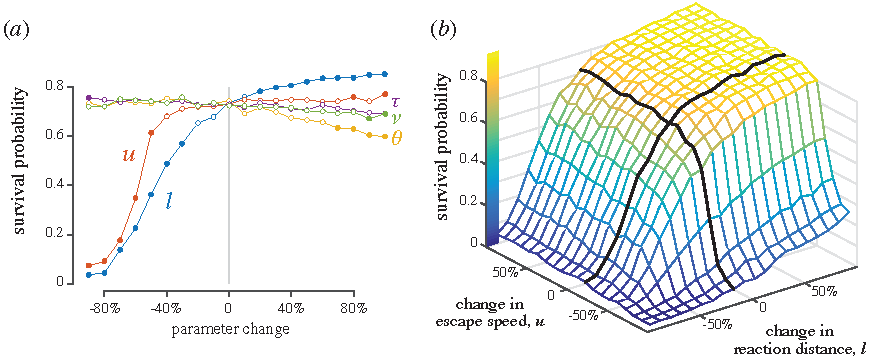
\includegraphics[width=5.5in]{fig_sensitivity}
\caption{Parameter analysis of the probabilistic, agent-based model to examine the effects of parameters on escape probability.   
(\textit{a}) We individually varied the mean parameter value among simulations by manipulating the distribution (Fig. \ref{fig_PDF}) of our measurements (see Table \ref{table} for parameter definitions and values). 
Each point represents the survival probability of prey among 1000 simulations and filled circles denote a significant difference (KS-test: P < 0.05) from the observed probability.
Simulations that varied in escape angle ($\theta$) differed by a interval of 0.127 rad.
(\textit{b}) Variation in escape probability was examined with respect to both escape speed and reaction distance.
The same simulation results are shown with respect to changes in escape speed (\textit{c}) and reaction distance (\textit{d}). All simulations used an adult predator, although similar results were obtained with a juvenile predator (Fig. S1).
}
\label{fig_sense}
\end{figure}

\pagebreak



\end{document}
